To address \textbf{RQ1} regarding dynamic preference elicitation, the system is built around an event-driven conversational workflow. This workflow manages the multi-turn, mixed-initiative dialogue between the user and the agent. The entire conversation is modeled as a graph of events, where nodes represent different states and steps in the process, as illustrated in Figure~\ref{FIG:EVENT_WORKFLOW}.

\begin{figure}[Workflow Event Graph]{FIG:EVENT_WORKFLOW}{An event graph diagram representing the conversational workflow.}
    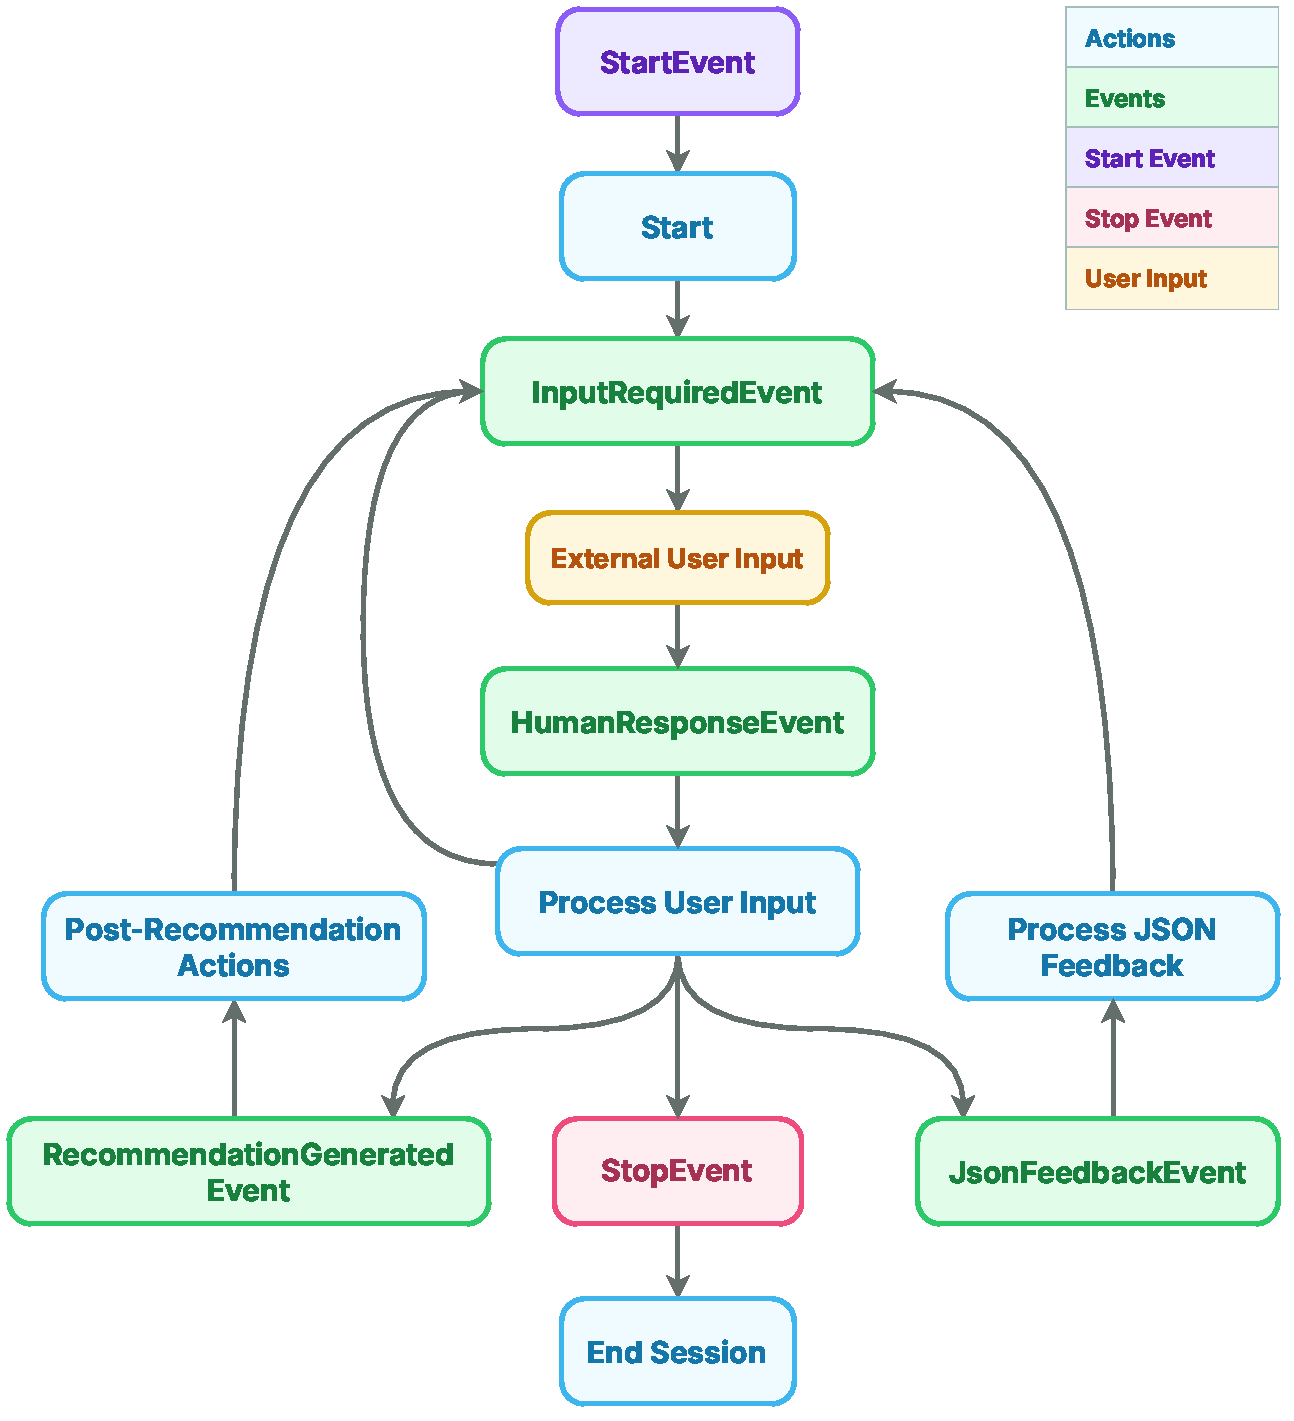
\includegraphics[width=\textwidth]{hybrid_crs_eventflow.pdf}
\end{figure}

At each turn, the \ac{llm} processes the user's natural language input within the context of the conversation history. Based on this context, the workflow's underlying logic determines the next action. This could be to ask a clarifying question to elicit more specific preferences (e.g., asking about a genre if the user's intent is vague), or to trigger a recommendation. This decision is not pre-scripted but is guided by the \ac{llm}'s reasoning capabilities. To interact with the system's other components, the workflow leverages Function Calling. This allows the \ac{llm} to autonomously decide when to call the specialized recommendation or explanation modules, passing the relevant information from the conversation as arguments.